\documentclass[11pt]{article}

\usepackage[letterpaper,margin=0.75in]{geometry}
\usepackage{booktabs}
\usepackage{graphicx}
\usepackage{listings}

\setlength{\parindent}{1.4em}

\begin{document}

\lstset{
  language=Python,
  basicstyle=\small,          % print whole listing small
  keywordstyle=\bfseries,
  identifierstyle=,           % nothing happens
  commentstyle=,              % white comments
  stringstyle=\ttfamily,      % typewriter type for strings
  showstringspaces=false,     % no special string spaces
  numbers=left,
  numberstyle=\tiny,
  numbersep=5pt,
  frame=tb,
}

\title{Lab 2 Report}

\author{Nate Fox}

\date{}

\maketitle

\section{Reliable Transport}
\subsection{Sender Implementation}
My sender implementation can be broken down into three main functions: sending TCP segments, handling ACKs, and retransmitting.
\paragraph{Sending TCP Segments}
When an application passes data to the TCP send function, my implementation writes that data to its send buffer and then calls a subroutine that sends all data that is both available (i.e. not yet sent) and within the window that limits the number of packets that can be sent at one time. The subroutine breaks down the available data into segments no bigger than the maximum segment size. It then records the current time (which is used to implement the dynamic retransmission timer) and calls another subroutine that sends the packet and starts the retransmission timer.
\begin{lstlisting}
def send(self,data):
	self.send_buffer.put(data)
	self.send_available()

def send_available(self):
	# While there is available data within the window
	while (self.send_buffer.available() is not 0) and \
	(self.send_buffer.outstanding() + self.mss <= self.window):
		# Get the largest amout of data allowed
		tcp_packet, start_sequence = self.send_buffer.get(self.mss)
		# Record send time for RTT estimate
		self.rtt.record_send_time(start_sequence, len(tcp_packet), \
			Sim.scheduler.current_time())
		# Send packet
		self.send_packet(tcp_packet, start_sequence)

def send_packet(self,data,sequence):
	packet = TCPPacket(source_address=self.source_address,
		   source_port=self.source_port,
		   destination_address=self.destination_address,
		   destination_port=self.destination_port,
		   body=data, sequence=sequence,ack_number=self.ack)
	# send the packet
	self.transport.send_packet(packet)
	# set a timer
	if not self.timer:
		self.timer = Sim.scheduler.add(delay=self.rtt.get_timeout(), \
			event='retransmit', handler=self.retransmit)
\end{lstlisting}
\pagebreak
\paragraph{Handling ACKs}
When the sender receives an incoming ACK, the first thing I do is check to see if it is larger than the largest ACK I have received so far. If it is not, then I ignore it, because that data has already been ACKed. If the incoming ACK is larger, I first record the current time to update the dynamic retransmission timer. I then restart the retransmission timer, in accordance with section 5.3 of RFC 2988. If all outstanding data has been acknowledged, I cancel the timer, in accordance with section 5.2 of RFC 2988. I then update the largest ACK received so far and update the buffer. With the buffer updated, new data may be available, so I call the subroutine to send available data.
\begin{lstlisting}
def handle_ack(self,packet):
	# If new ACK
	if packet.ack_number > self.sequence:
		# Record ACK time for RTT estimate
		self.rtt.record_ack_time(packet.ack_number, \
			Sim.scheduler.current_time())
		# Restart timer
		self.cancel_timer()
		self.timer = Sim.scheduler.add(delay=self.rtt.get_timeout(), \
			event='retransmit', handler=self.retransmit)
		# Update self.sequence (largest sequence number ACKed so far)
		self.sequence = packet.ack_number
		# Update buffer
		self.send_buffer.slide(packet.ack_number)
		# If all outstanding data is acknowledged, cancel timer
		if self.send_buffer.outstanding() == 0:
			self.cancel_timer()
		# Send available data
		self.send_available()
\end{lstlisting}
\paragraph{Retransmitting Segments}
When the retransmission timer fires, I clear the RTT clock's send times so that retransmitted segments don't affect the estimated RTT. I also perform exponential backoff, which doubles the RTO in accordance with section 5.5 of RFC 2988. I restart the retransmission timer to expire after RTO seconds, in accordance with section 5.6 of RFC 2988. I then retransmit the earliest segment that has not been acknowledged.
\begin{lstlisting}
def retransmit(self,event):
	# Clear RTT clock send times, perform exponential backoff
	self.rtt.clear_send_times()
	self.rtt.exponential_backoff()
	# Restart timer to expire after RTO seconds
	self.timer = Sim.scheduler.add(delay=self.rtt.get_timeout(), \
		event='retransmit', handler=self.retransmit)
	# Resend earliest unACKed segment
	tcp_packet, start_sequence = self.send_buffer.resend(self.mss)
	self.send_packet(tcp_packet, start_sequence)
\end{lstlisting}
\pagebreak
\subsection{Receiver Implementation}
My receiver implementation is fairly simple: it sorts the data that it receives, sends ordered data to the application, and sends an ACK back to the sender. When I receive a packet, I put it in the buffer. The buffer takes care of ignoring duplicate data and putting the data in order. I then ask the buffer for the data that is in the correct order and I send that data to the application. Then I update the ACK value and send an ACK to the sender.
\begin{lstlisting}
def handle_data(self,packet):
	# Put packet in buffer
	self.receive_buffer.put(packet.body, packet.sequence)
	# Send all ordered data to the application
	ordered_data, start_sequence = self.receive_buffer.get()
	self.app.receive_data(ordered_data)
	# Update ACK value and send ACK
	self.ack = start_sequence + len(ordered_data)
	self.send_ack()

def send_ack(self):
	packet = TCPPacket(source_address=self.source_address,
			   source_port=self.source_port,
			   destination_address=self.destination_address,
			   destination_port=self.destination_port,
			   sequence=self.sequence,ack_number=self.ack)
	# send the packet
	self.transport.send_packet(packet)
\end{lstlisting}
\subsection{Tests}
To test with a constant timer of 1 second, I modified my RoundTripTimer's get\_timeout() function to always return 1.
\begin{lstlisting}
def get_timeout(self):
	return 1 # Fixed timer
\end{lstlisting}
To set up the network for the tests, I created test-network.txt and configured transfer.py to load this network.
\begin{lstlisting}
# n1 -- n2
#
n1 n2
n2 n1

# link configuration
n1 n2 10Mbps 10ms
n2 n1 10Mbps 10ms
\end{lstlisting}
I also modified transfer.py to accept window size as a command line parameter. For example, running ``python transfer.py -f test.txt -l 0.10 -w 3000'' transfers the file test.txt with a simulated loss of 10\% and a window size of 3000 bytes.
\pagebreak
\subsubsection{Transfer test.txt with 3000-byte window}
\paragraph{0\% Loss}
python transfer.py -f test.txt -l 0.0 -w 3000
\begin{lstlisting}
0 n1 (1) sending TCP segment to 2 for 0
0 n1 (1) sending TCP segment to 2 for 1000
0 n1 (1) sending TCP segment to 2 for 2000
0.0108 n2 (2) received TCP segment from 1 for 0
0.0108 application got 1000 bytes
0.0108 n2 (2) sending TCP ACK to 1 for 1000
0.0116 n2 (2) received TCP segment from 1 for 1000
0.0116 application got 1000 bytes
0.0116 n2 (2) sending TCP ACK to 1 for 2000
0.0124 n2 (2) received TCP segment from 1 for 2000
0.0124 application got 1000 bytes
0.0124 n2 (2) sending TCP ACK to 1 for 3000
0.0208 n1 (1) received TCP ack from 2 for 1000
0.0208 n1 (1) sending TCP segment to 2 for 3000
0.0216 n1 (1) received TCP ack from 2 for 2000
0.0216 n1 (1) sending TCP segment to 2 for 4000
0.0224 n1 (1) received TCP ack from 2 for 3000
0.0224 n1 (1) sending TCP segment to 2 for 5000
...
0.0624 n1 (1) sending TCP segment to 2 for 9000
0.0632 n1 (1) received TCP ack from 2 for 8000
0.064 n1 (1) received TCP ack from 2 for 9000
0.0732 n2 (2) received TCP segment from 1 for 9000
0.0732 application got 1000 bytes
0.0732 n2 (2) sending TCP ACK to 1 for 10000
0.0832 n1 (1) received TCP ack from 2 for 10000
\end{lstlisting}
This test shows us that when there is no packet loss, everything works smoothly. N1 sends the first 3000 bytes (limited by window of length 3000) in 1000-byte segments (limited by maximum segment size). N1 can't send another segment until it receives the ACK from 2 for 1000, at which point N1 sends the next segment (sequence 3000). The retransmission timer is never fired, and the entire process takes only 0.08 s.
\paragraph{10\% Loss}
python transfer.py -f test.txt -l 0.10 -w 3000
\begin{lstlisting}
0 n1 (1) sending TCP segment to 2 for 0
0 n1 (1) sending TCP segment to 2 for 1000
0 n1 (1) sending TCP segment to 2 for 2000
0.0108 n2 (2) received TCP segment from 1 for 0
0.0108 application got 1000 bytes
0.0108 n2 (2) sending TCP ACK to 1 for 1000
0.0116 n2 (2) received TCP segment from 1 for 2000
0.0116 application got 0 bytes
0.0116 n2 (2) sending TCP ACK to 1 for 1000
0.0208 n1 (1) received TCP ack from 2 for 1000
0.0208 n1 (1) sending TCP segment to 2 for 3000
0.0316 n2 (2) received TCP segment from 1 for 3000
0.0316 application got 0 bytes
0.0316 n2 (2) sending TCP ACK to 1 for 1000
0.0416 n1 (1) received TCP ack from 2 for 1000
1.0208 n1 (1) retransmission timer fired
1.0208 n1 (1) sending TCP segment to 2 for 1000
1.0316 n2 (2) received TCP segment from 1 for 1000
1.0316 application got 3000 bytes
1.0316 n2 (2) sending TCP ACK to 1 for 4000
1.0416 n1 (1) received TCP ack from 2 for 4000
...
1.0748 n2 (2) sending TCP ACK to 1 for 10000
1.0832 n1 (1) received TCP ack from 2 for 8000
1.084 n1 (1) received TCP ack from 2 for 9000
1.0848 n1 (1) received TCP ack from 2 for 10000
\end{lstlisting}
During this test, we can see that the second segment (sequence 1000) was dropped and had to be retransmitted. N2 sends ACKs for 1000 three times before the timer is fired and the sender resends sequence 1000. N2 received sequence 0, sequence 2000, and sequence 3000, but can only ACK 1000 because that is the lowest byte that it has not yet received. The timer is fired and N1 retransmits sequence 1000. N2 receives it and sends back an ACK for 4000, because now 4000 is the lowest byte that is has not yet received. The remainder of the file transfer goes smoothly, and the entire process takes about 1.08 s.
\paragraph{20\% Loss}
python transfer.py -f test.txt -l 0.20 -w 3000
\begin{lstlisting}
...
1.0216 n1 (1) retransmission timer fired
1.0216 n1 (1) sending TCP segment to 2 for 2000
...
3.0216 n1 (1) retransmission timer fired
3.0216 n1 (1) sending TCP segment to 2 for 2000
...
4.064 n1 (1) retransmission timer fired
4.064 n1 (1) sending TCP segment to 2 for 6000
...
4.0748 n2 (2) sending TCP ACK to 1 for 7000
6.064 n1 (1) retransmission timer fired
6.064 n1 (1) sending TCP segment to 2 for 6000
...
8.064 n1 (1) retransmission timer fired
8.064 n1 (1) sending TCP segment to 2 for 6000
...
8.1072 n1 (1) received TCP ack from 2 for 10000
\end{lstlisting}
The retransmission timer fired five times during this test. Some segments were dropped (like sequence 2000) and some ACKs were dropped (like the ACK for 7000), resulting in segments 2000 and 6000 being sent multiple times. The entire process takes about 8.1 s.
\paragraph{50\% Loss}
python transfer.py -f test.txt -l 0.50 -w 3000
\begin{lstlisting}
...
30.1248 n1 (1) received TCP ack from 2 for 10000
\end{lstlisting}
For this test, the timer fired 17 times, causing the entire process to take about 30.1 s.
\subsubsection{Transfer internet-architecture.pdf with 10000-byte window}
\paragraph{0\% Loss}
python transfer.py -f internet-architecture.pdf -l 0.0 -w 10000
\begin{lstlisting}
...
1.084416 n1 (1) received TCP ack from 2 for 514520
\end{lstlisting}
With no packet loss, the entire file transfer took about 1.08 s.
\paragraph{10\% Loss}
python transfer.py -f internet-architecture.pdf -l 0.10 -w 10000
\begin{lstlisting}
...
41.694432 n1 (1) received TCP ack from 2 for 514520
\end{lstlisting}
With 10\% loss, the timer was fired 35 times and the file transfer took about 41.7 s.
\paragraph{20\% Loss}
python transfer.py -f internet-architecture.pdf -l 0.20 -w 10000
\begin{lstlisting}
...
87.993216 n1 (1) received TCP ack from 2 for 514520
\end{lstlisting}
With 20\% loss, the timer was fired 66 times and the file transfer took about 88.0 s.
\paragraph{50\% Loss}
python transfer.py -f internet-architecture.pdf -l 0.50 -w 10000
\begin{lstlisting}
...
666.2232 n1 (1) received TCP ack from 2 for 514520
\end{lstlisting}
With 50\% loss, the timer was fired 382 times and the file transfer took about 666.2 s.
\paragraph{Result Table}

\begin{tabular}{lll}
	\toprule
	Loss \% & Timer Fired & Transfer Time\\
	\midrule
	0 & 0 & 1.08\\
	10 & 35 & 41.7\\
	20 & 66 & 80.0\\
	50 & 382 & 666.2\\
	\bottomrule
\end{tabular}

\section{Dynamic Retransmission Timer}
\subsection{Implementation}
To implement the dynamic retransmission timer, I created a RoundTripTimer object to keep track of the estimated round trip time and the estimated deviation.
\begin{lstlisting}
class RoundTripTimer(object):
	
	def __init__(self):
		self.samples = {}
		self.rto = 1
		self.estimated_rtt = 1
		self.dev_rtt = 0
		self.alpha = 0.125
		self.beta = 0.25
		self.output_file = open("timeouts.txt", "w")

	def get_timeout(self):
		self.output_file.write(str(self.rto) + "\n")
		return self.rto

	def record_send_time(self, sequence, length, time):
		self.samples[sequence+length] = time

	def record_ack_time(self, ack, time):
		if ack not in self.samples:
			return
		sample_rtt = time - self.samples[ack]
		self._update_estimates(sample_rtt)

	def exponential_backoff(self):
		self.rto = self.rto * 2

	def clear_send_times(self):
		self.samples = {}

	def _update_estimates(self, sample_rtt):
		self.estimated_rtt = ((1 - self.alpha) * self.estimated_rtt) + \
			(self.alpha * sample_rtt)
		self.dev_rtt = ((1 - self.beta) * self.dev_rtt) + \
			(self.beta * abs(sample_rtt - self.estimated_rtt))
		self.rto = self.estimated_rtt + (4 * self.dev_rtt)
\end{lstlisting}
Whenever I send a TCP segment for the first time, I record the sequence number, the length, and the current simulated time. When I receive an ACK, I find the recorded time for the ACKed segment to get a sample round trip time. I use that sample to update the estimated round trip time, estimated deviation, and the RTO. Whenever my TCP implementation sets a timer, it calls get\_timeout() on its RoundTripTimer instance, which returns the RTO and writes it to a file. Whenever my retransmission timer goes off, I clear the send times and perform exponential backoff. Once I get another sample RTT measurement, I recompute the RTO based on the estimated RTT and deviation, thus collapsing RTO back down after it has been subject to exponential backoff (See RFC 2988 Section 5).
\subsection{Tests}
\paragraph{0\% Loss}
python transfer.py -f internet-architecture.pdf -l 0.0 -w 10000
\begin{lstlisting}
...
1.084416 n1 (1) received TCP ack from 2 for 514520
\end{lstlisting}
With a 0\% loss, the time is the same as it was with a constant 1 second timer, because the timer is never fired. The timer very quickly converges to a value of about 0.0208 seconds, but it never gets fired.

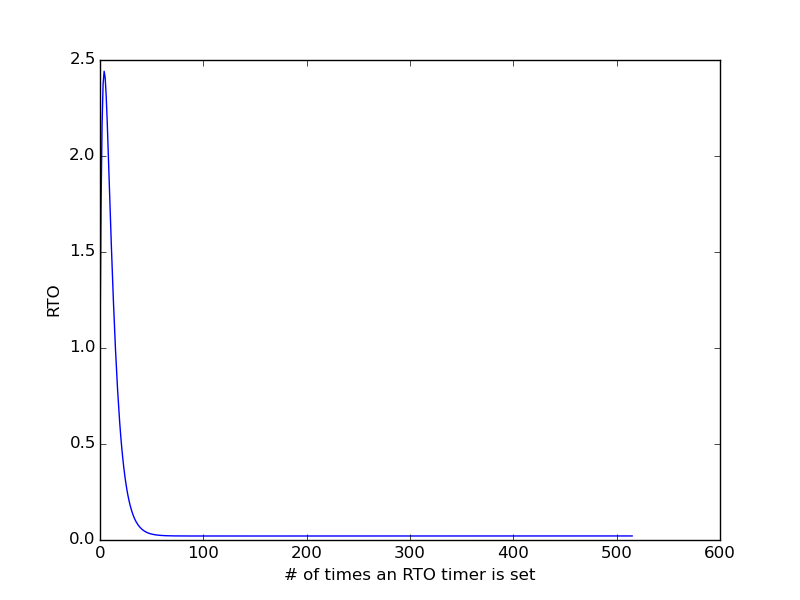
\includegraphics[width=10cm]{../graphs/timeout_0.png}
\pagebreak
\paragraph{10\% Loss}
python transfer.py -f internet-architecture.pdf -l 0.10 -w 10000
\begin{lstlisting}
...
1.0672 n1 (1) sending TCP segment to 2 for 27000
...
2.32796755566 n1 (1) retransmission timer fired
2.32796755566 n1 (1) sending TCP segment to 2 for 27000
...
6.82317957004 n1 (1) sending TCP segment to 2 for 486000
...
6.8585526009 n1 (1) retransmission timer fired
6.8585526009 n1 (1) sending TCP segment to 2 for 486000
...
6.9277686009 n1 (1) received TCP ack from 2 for 514520
\end{lstlisting}
With a 10\% loss, the transfer took about 6.93 s with a dynamic timer, whereas it took about 41.7 s with a constant timer. The timer converges to a value of about 0.028 seconds, but you can see several bumps in the graph where exponential backoff occurs. The retransmission timer fired 36 times, and each time the RTO was doubled. Once a successful segment transfer gave me a new sample RTT measurement, the RTO was recomputed, causing the RTO to collapse back down to where it was before the exponential backoff.

The debug output above shows that the timer when sequence 27000 was sent was set at about 1.2 seconds. Later, when sequence 486000 was sent, the timer was about 0.03 seconds.

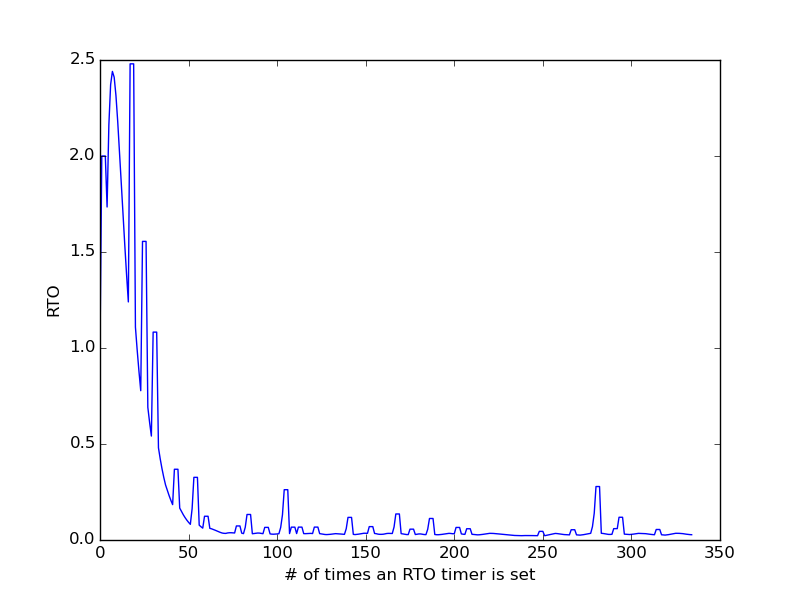
\includegraphics[width=10cm]{../graphs/timeout_10.png}
\paragraph{20\% Loss}
python transfer.py -f internet-architecture.pdf -l 0.20 -w 10000
\begin{lstlisting}
...
19.5059682831 n1 (1) sending TCP segment to 2 for 45000
...
53.9291270517 n1 (1) retransmission timer fired
53.9291270517 n1 (1) sending TCP segment to 2 for 45000
...
78.3457841376 n1 (1) received TCP ack from 2 for 514520
\end{lstlisting}
With a 20\% loss, the transfer took about 78.3 s with a dynamic timer, whereas it took about 80 s with a constant timer. In this specific case, the time difference was pretty small. One reason for this is that exponential backoff occurred multiple times in a row near the beginning, which made the RTO peak at nearly 35 seconds. Eventually the RTO converged to about 0.118 seconds.

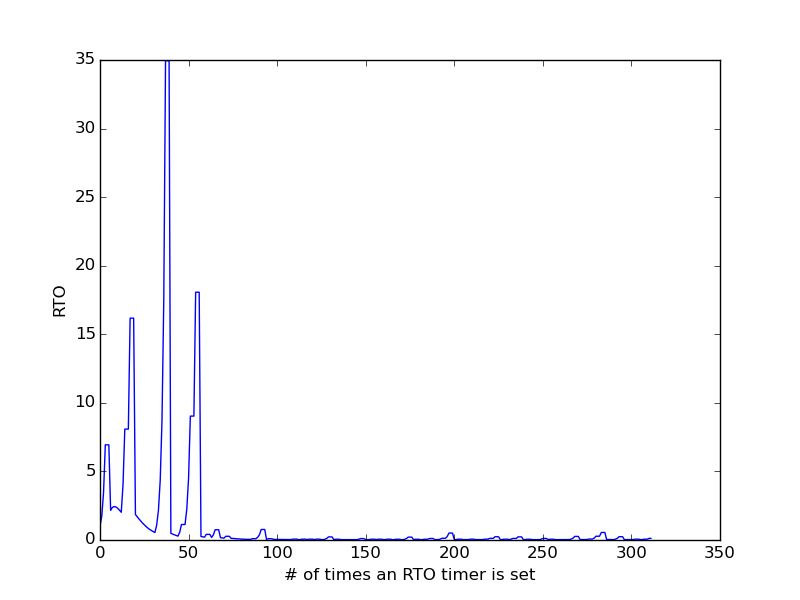
\includegraphics[width=10cm]{../graphs/timeout_20.png}
\paragraph{50\% Loss}
python transfer.py -f internet-architecture.pdf -l 0.50 -w 10000
\begin{lstlisting}
...
6154.20561751 n1 (1) received TCP ack from 2 for 514520
\end{lstlisting}
With a 50\% loss, I had to cap the RTO at 60 seconds to contain it. It still took 6154 s, whereas it took only 666.2 s with a constant timer. With such a high loss rate, exponential backoff occurs too frequently and it collapses back too infrequently. It never converged.

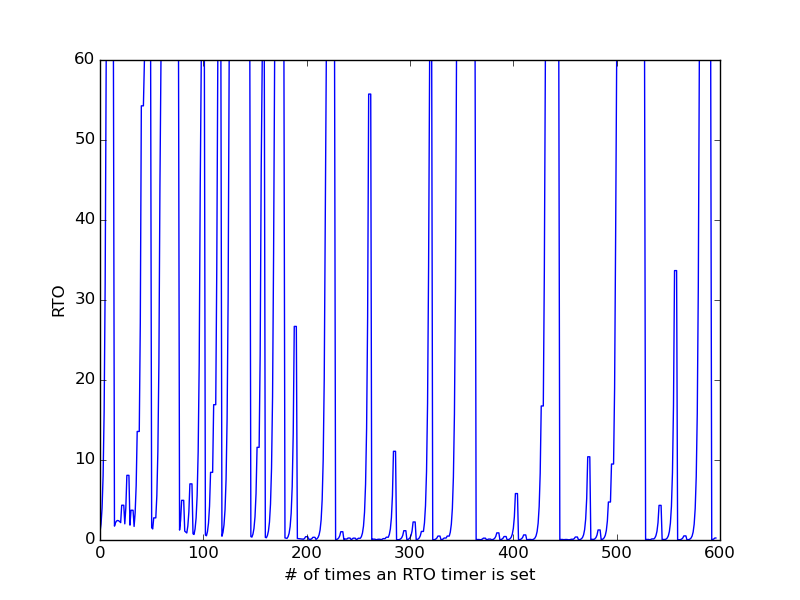
\includegraphics[width=10cm]{../graphs/timeout_50.png}

\pagebreak
\section{Experiments}
To determine the affect that window size has on transfer time, I am going to transfer the internet-architecture.pdf file over a single link (10 Mbps bandwidth, 10 ms propagation delay, 100-packet queue, loss rate 0\%) and use variable window sizes. Before running these experiments, I changed the links in my test network to have queues that could hold at most 100 packets.
\begin{lstlisting}
# n1 -- n2
#
n1 n2
n2 n1

# link configuration
n1 n2 10Mbps 10ms 100pkts
n2 n1 10Mbps 10ms 100pkts
\end{lstlisting}
I also changed my TCP implementation to write the current simulated time to a file every time a packet is sent. Since all packets are placed in the send buffer at time 0, the time that a packet is sent represents the amount of time it waited in the buffer. The loss for these experiments will be set to 0\%, so each packet will be sent only once. The data written to this file will be used to determine the average queueing delay.
\begin{lstlisting}
def send_packet(self,data,sequence):
	...
	self.queue_file.write(str(Sim.scheduler.current_time()) + "\n")
	...
\end{lstlisting}
\subsection{Results}

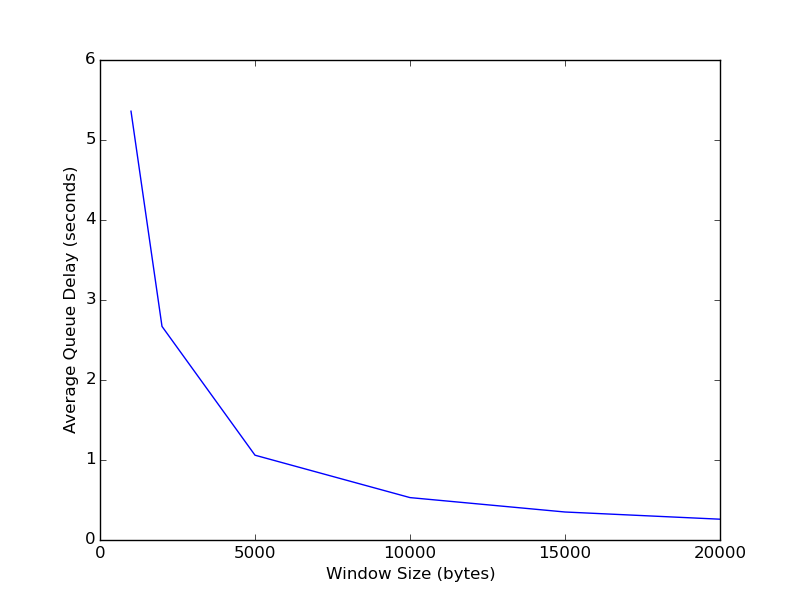
\includegraphics[width=12cm]{../graphs/queue_delay_graph.png}

\paragraph{Queueing Delay}
From the above graph, we can see that the average queueing delay is inversely proportional to the window size. As the window size approaches infinity, the queueing delay approaches zero. For this particular experiment, the only queueing delay is caused by the time that a segment is waiting in the send buffer. As the window gets smaller, the segments have to be in the send buffer for longer, hence the inverse relationship.

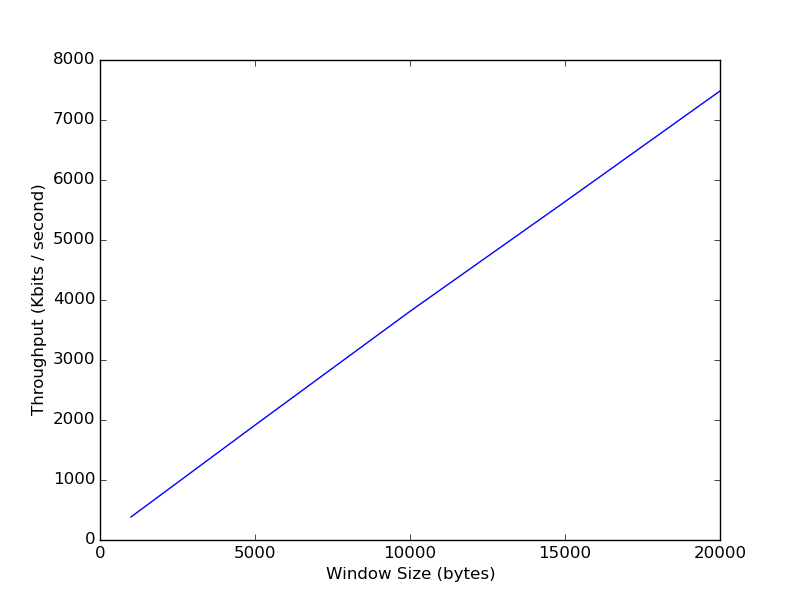
\includegraphics[width=12cm]{../graphs/throughput_graph.png}
\paragraph{Throughput}
From this graph, we can see that the throughput is directly proportional to the window size. When the window size increases, TCP can send more data at a time, thus increasing throughput.

\end{document}
